\documentclass{article}
\usepackage[utf8]{inputenc}
\usepackage[margin=1in,left=1.5in,includefoot]{geometry}
\usepackage{booktabs}
\usepackage{graphicx}

% Header & Footer Stuff

\usepackage{fancyhdr}
\pagestyle{fancy}
\lhead{Fundamentos de Robótica Intelixente}
\rhead{614G030302425}
% \fancyfoot{}
% \lfoot{Pablo Chantada Saborido \& José Romero Conde}
% \fancyfoot[R]{}

% The Main Document
\begin{document}
\begin{center}
    \LARGE\bfseries PRÁCTICA III\\
    \small Pablo Chantada Saborido \& José Romero Conde
    \line(1,0){430}
\end{center}


\subsection*{Ejercicio 1}

Este ejercicio implementa un controlador básico del robot Robobo mediante teclado.
$$
\text{Teclas de control: } &\begin{cases}
\text{w} &\rightarrow \text{Avance} \
\text{s} &\rightarrow \text{Retroceso} \
\text{a} &\rightarrow \text{Giro izquierda} \
\text{d} &\rightarrow \text{Giro derecha} \
\text{q} &\rightarrow \text{Detener y salir} \
\end{cases}
$$
El sistema utiliza la biblioteca pynput para capturar los eventos de teclado y controla el robot estableciendo velocidades a las ruedas (SPEED=10)(\text{SPEED} = 10)
(SPEED=10).


\subsection*{Ejercicio 2}

Este ejercicio permite controlar el robot Robobo mediante comandos de texto introducidos en una interfaz gráfica.
$$\begin{align}
\text{Movimientos básicos: } &\begin{cases}
\text{forward} &\rightarrow (v, v) \
\text{back} &\rightarrow (-v, -v) \
\text{left} &\rightarrow (-v, v) \
\text{right} &\rightarrow (v, -v)
\end{cases}
\end{align}$$
$$\begin{align}
\text{Movimientos compuestos: } &\begin{cases}
\text{forward-left} &\rightarrow (v/2, v) \
\text{forward-right} &\rightarrow (v, v/2) \
\text{back-left} &\rightarrow (-v, -v/2) \
\text{back-right} &\rightarrow (-v/2, -v)
\end{cases}
\end{align}$$
Admite parámetros:

speed X: Establece velocidad a XX
X
time Y: Establece duración a YY
Y segundos

\subsection*{Ejercicio 2b}

Extensión del ejercicio 2 que utiliza reconocimiento de voz en español y añade control de emociones y LEDs.
$$\begin{align}
\text{Movimientos: } &\begin{cases}
\text{delante} \
\text{atrás} \
\text{izquierda} \
\text{derecha}
\end{cases} \quad
\text{Emociones: } \begin{cases}
\text{feliz} \
\text{triste} \
\text{enfadado}
\end{cases} \quad
\text{Colores LED: } \begin{cases}
\text{rojo} \
\text{verde} \
\text{azul}
\end{cases}
\end{align}$$
Utiliza la biblioteca speech\_recognition con reconocimiento Google (language="es").

\subsection*{Ejercicio 3}

\begin{figure}[h]
	\centering
	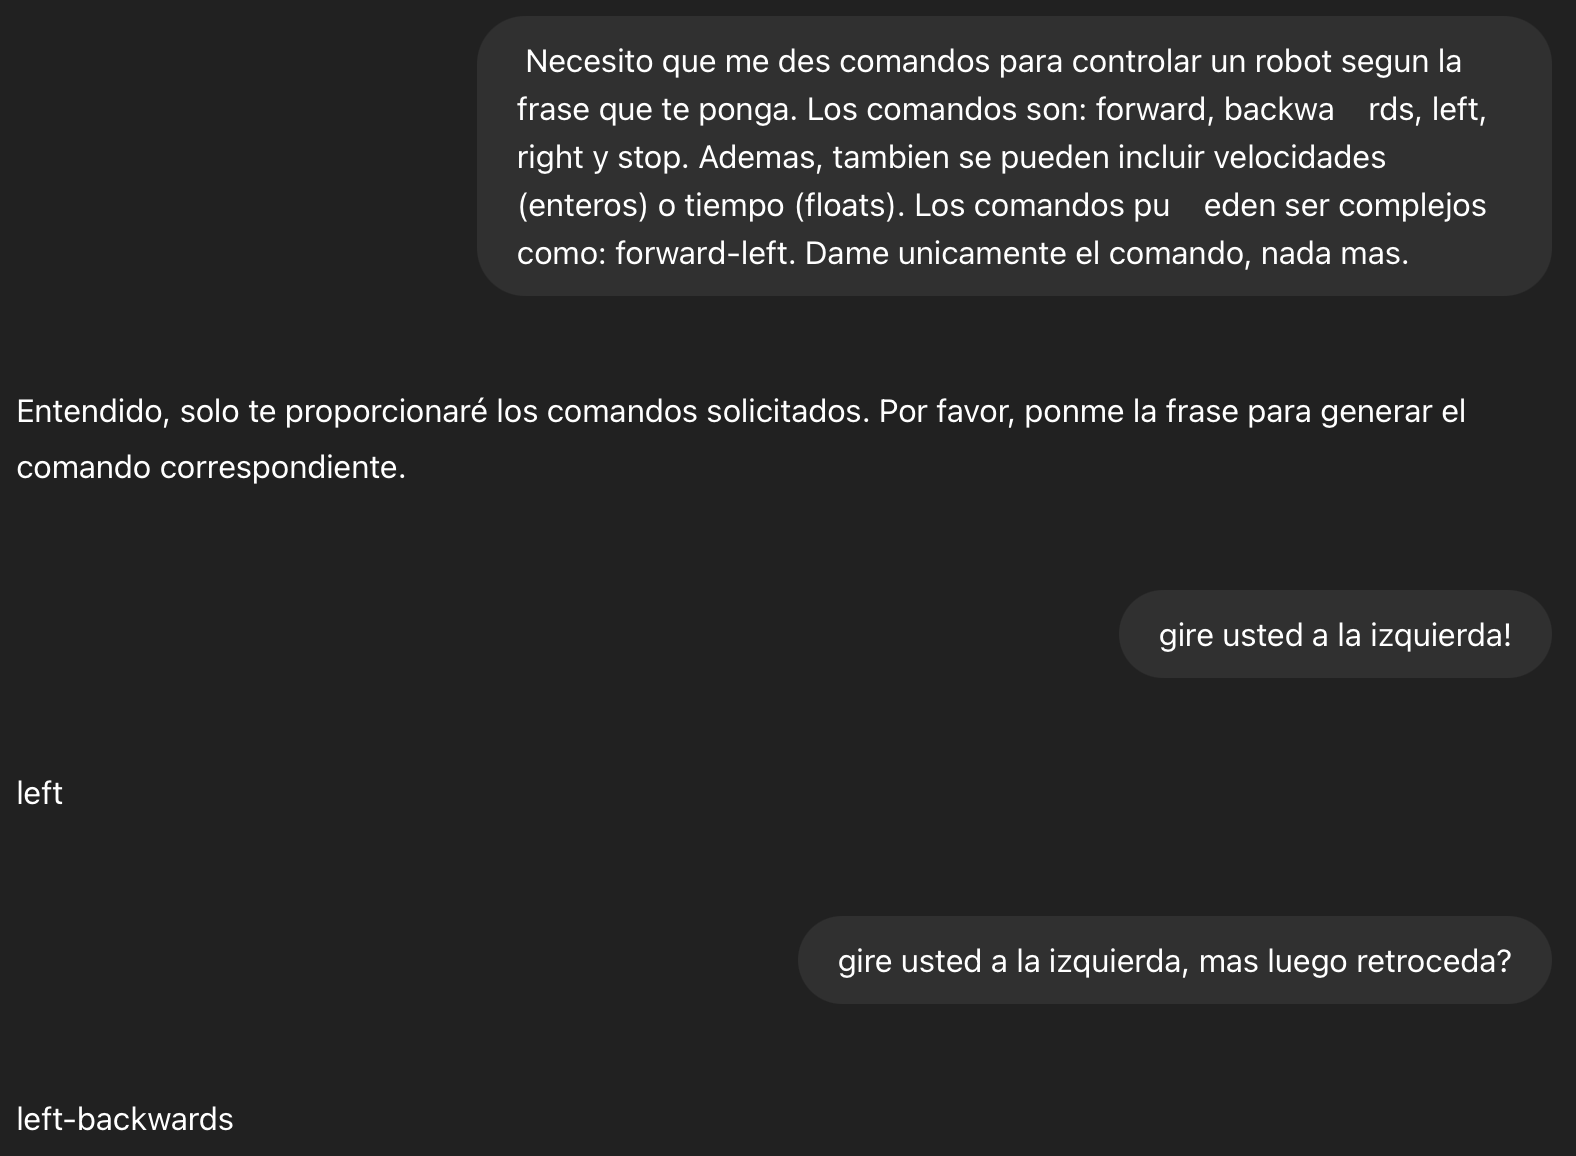
\includegraphics[width=0.7\linewidth]{captura}
	\caption{chatgpt}
	\label{fig:captura}
\end{figure}


\subsection*{Ejercicio 4}

Este ejercicio integra ChatGPT para interpretar comandos en lenguaje natural y convertirlos en instrucciones para el robot.
$$\begin{aligned}
	\text{Entrada:} &\text{ "Avanza un poco"} \
	\text{Procesamiento ChatGPT} &\downarrow \
	\text{Salida:} &\text{ "forward"}
\end{aligned}$$
El sistema utiliza un prompt específico para extraer comandos válidos para el robot a partir del lenguaje natural.

\subsection*{Ejercicio 5}

Este ejercicio avanza en la integración con ChatGPT, generando un vector de control completo para el robot.
$$\begin{aligned}
	\text{Vector de control:} &[v_x, v_y, \text{emoción}, \text{sonido}, \text{texto}] \
	\text{Ejemplo:} &[50, 50, \text{"happy"}, \text{"happy"}, \text{"¡Avanzando!"}]
\end{aligned}$$
Donde:

vx,vy∈[−100,100]v_x, v_y \in [-100, 100]
vx​,vy​∈[−100,100] son las velocidades de las ruedas

emocioˊn∈{"happy","sad","angry"}\text{emoción} \in \{\text{"happy"}, \text{"sad"}, \text{"angry"}\}
emocioˊn∈{"happy","sad","angry"}
sonido∈{"happy","sad","angry"}\text{sonido} \in \{\text{"happy"}, \text{"sad"}, \text{"angry"}\}
sonido∈{"happy","sad","angry"}
texto\text{texto}
texto es un mensaje que el robot pronunciará


El controlador ejecuta todos los parámetros y detiene el robot después de 3 segundos por seguridad.

\end{document}

